% ===================================================================== PARTE I
\chapter{El problema en palabras simples}

\section{Pagar es un acto colectivo}
Cada día una persona recibe su sueldo, paga el arriendo, le transfiere dinero a un
familiar y abona la cuota de un crédito. Una empresa cobra a sus clientes, paga a sus
proveedores y paga la nómina. Hoy casi todo eso ocurre en \term{sistemas de pagos
digitales}: transferencias que salen de una cuenta y llegan a otra en segundos. En
Colombia el ejemplo más reciente es \term{Bre-B}, el sistema de pagos inmediatos
interoperable promovido por el Banco de la República: cualquier persona puede pagarle
a otra en cualquier entidad, a cualquier hora.

Lo importante para este proyecto es una observación sencilla: \textbf{nadie paga solo}.
Lo que yo puedo pagar depende de lo que me pagaron a mí. Si mi empleador se retrasa,
yo me retraso con el arriendo; si un cliente grande no le paga a una empresa, la
empresa se retrasa con sus proveedores y con su nómina. Los pagos forman una
\term{red}: una telaraña de quién le paga a quién.

\section{Liquidez: tener dinero \emph{ahora}}
Dos palabras que suelen confundirse:
\begin{itemize}
\item \term{Solvencia}: tener más de lo que se debe, en total. Una tienda con mucho
inventario es solvente.
\item \term{Liquidez}: tener dinero disponible \emph{en el momento} en que hay que
pagar. La misma tienda puede no tener efectivo hoy para pagar el arriendo, aunque
sea solvente.
\end{itemize}
A la falta de liquidez la llamaremos \term{déficit}: cuánto dinero falta para cubrir
los pagos del momento. Un déficit pequeño se resuelve (se pide prestado, se recorta un
gasto, se espera el siguiente ingreso). Un déficit demasiado grande termina en un
\term{impago}: no se paga lo que se debía.

\section{El efecto dominó}
Si una entidad deja de pagar, quienes esperaban ese dinero reciben menos. Algunos lo
absorben con su colchón; otros no, y también dejan de pagar. Un problema local se
vuelve una \term{cascada}. Al riesgo de que eso pase se le llama \term{riesgo
sistémico}: no es el riesgo de una entidad, es el riesgo del \emph{sistema}. La crisis
financiera de 2008 hizo famoso el concepto: entidades ``demasiado conectadas para
caer'' cuya caída arrastraba a muchas otras.

\section{El ritmo de los pagos}
Los pagos no llegan de forma continua; llegan en \term{ciclos}. La nómina se paga
cada quince días o cada mes; las facturas, a 30 o 60 días; las cuotas de un crédito,
en una fecha fija. Si una persona recibe su sueldo el día 30 pero sus gastos fuertes
caen el día 15, vive dos semanas apretada: necesita un colchón mayor. Si dos
entidades que dependen una de la otra tienen ritmos \emph{desfasados}, el dinero
llega justo cuando ya no sirve. A esto lo llamaremos \term{desincronización}.

\begin{idea}[Una imagen]
Piense en un grupo de personas que se pasan baldes de agua en fila para apagar un
incendio. Si todos se mueven al mismo ritmo, el agua fluye. Si uno se adelanta o se
atrasa, los baldes se acumulan o se caen. La red de pagos es esa fila, pero con forma
de telaraña; el ritmo de cada uno es su ciclo de pagos.
\end{idea}

\section{Riesgo crediticio: ¿me van a pagar?}
Un banco que presta dinero se pregunta, para cada cliente: ¿cuál es la probabilidad de
que no pague su crédito en el próximo año? Esa probabilidad se llama \term{PD}
(\emph{probability of default}, probabilidad de impago). Para estimarla, los bancos
usan un \term{score crediticio}: un modelo estadístico que combina el ingreso, el
nivel de endeudamiento, el historial de moras, la antigüedad, el tipo de empleo, etc.
Esto lo hacen todos los bancos desde hace décadas.

Pero el score clásico mira a cada cliente \emph{aislado}. No ve que un cliente con buen
historial depende por completo del sueldo de una empresa que está en problemas, ni
que sus ingresos llegan desfasados de sus obligaciones.

\section{La pregunta del proyecto}
El proyecto tiene dos niveles:
\begin{enumerate}
\item \textbf{Riesgo sistémico} (tareas 1 a 5 de la propuesta): construir un modelo
físico-matemático de una red de pagos en el que el déficit se propaga, los ritmos de
pago se sincronizan o no, y las entidades caen cuando superan un umbral; y aprender a
predecir esos colapsos con aprendizaje automático.
\item \textbf{Riesgo crediticio} (tarea 6, la aplicación): llevar ese modelo a los
clientes de un banco y responder una pregunta medible:
\end{enumerate}
\begin{clave}[La pregunta central]
¿La \textbf{dinámica} de la red de pagos de los clientes (qué tan sincronizados están
sus ciclos de pago con los de quienes les pagan) aporta información sobre el impago
que ni el score clásico ni la \textbf{estructura estática} de la red capturan?
\end{clave}

% ---------------------------------------------------------------------------
\chapter{La idea física}

\section{Por qué la física tiene algo que decir}
La física estudia desde hace más de un siglo sistemas formados por muchas partes que
interactúan: átomos en un imán, neuronas en el cerebro, luciérnagas que terminan
destellando al unísono, generadores de una red eléctrica que deben girar a la misma
frecuencia. Tres ideas de esa tradición encajan con los pagos:

\begin{enumerate}
\item \textbf{Redes}. Las interacciones se describen con un grafo: puntos
(\term{nodos}) unidos por flechas (\term{aristas}). Aquí, los nodos son entidades o
clientes y las flechas son pagos.
\item \textbf{Osciladores acoplados}. Cada nodo tiene un ritmo propio; al
interactuar, los ritmos tienden a alinearse. El modelo de \term{Kuramoto} (1975)
describe exactamente esto y explica por qué, por encima de cierto acople, aparece la
sincronía colectiva.
\item \textbf{Umbrales y cascadas}. Un fusible aguanta hasta cierta corriente y luego
salta; un grano de arena más desata una avalancha. Los modelos de umbral describen
cómo un evento pequeño puede propagarse por toda una red.
\end{enumerate}

\section{Los tres ingredientes del modelo}
\begin{description}
\item[1. La red.] Una tabla $W$ que dice cuánto le paga cada entidad a cada otra por
ciclo. Es el ``mapa'' del sistema.
\item[2. El estado de cada nodo.] Dos números por entidad:
  \begin{itemize}
  \item su \term{déficit} $x_i$: cuánta liquidez le falta;
  \item su \term{fase} $\theta_i$: en qué punto de su ciclo de pagos está (como la
  aguja de un reloj que da una vuelta por ciclo).
  \end{itemize}
\item[3. Las reglas.] Cómo cambian esos números con el tiempo:
  \begin{itemize}
  \item el déficit tiende a corregirse solo, pero crece si quienes me pagan están en
  déficit (contagio);
  \item el ritmo de cada uno se ajusta al de quienes le pagan (sincronización);
  \item si el ingreso me llega desfasado, el déficit crece (la desincronización
  cuesta);
  \item si el déficit supera el colchón de la entidad, cae en impago y deja de pagar.
  \end{itemize}
\end{description}

\begin{figure}[h]
\centering
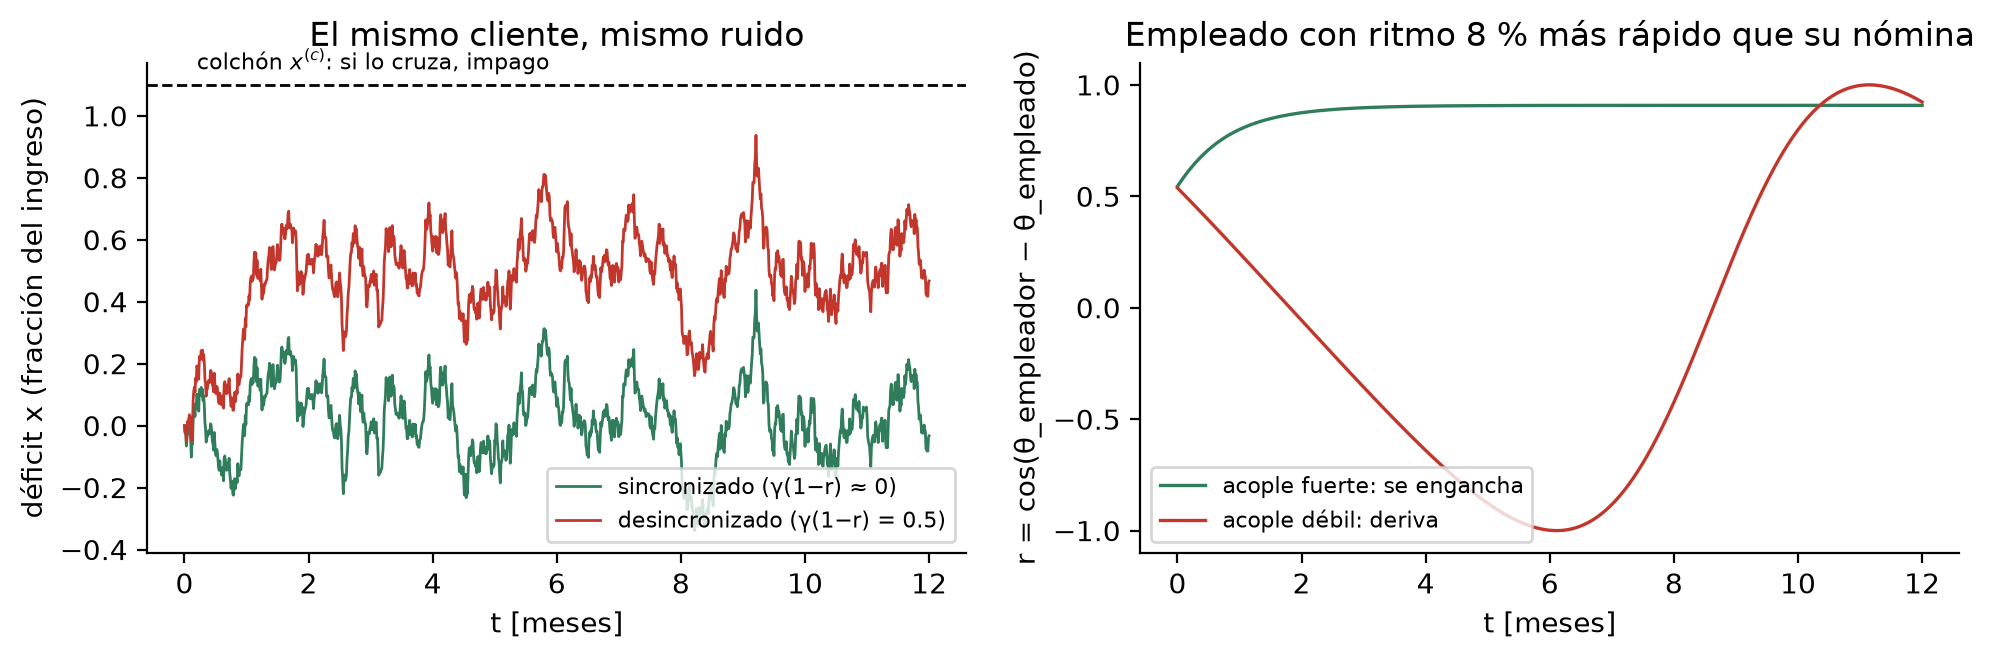
\includegraphics[width=\textwidth]{concepto_deficit_y_ritmo.png}
\caption{Izquierda: el mismo cliente con el mismo ruido; desincronizado, su déficit
vive más cerca del colchón y es más probable que lo cruce. Derecha: un empleado cuyo
ritmo natural es 8~\% más rápido que el de su nómina. Con acople fuerte se
``engancha'' (la coherencia $r$ se queda alta); con acople débil deriva y pasa por
momentos de desfase total ($r=-1$).}
\label{fig:concepto}
\end{figure}

\section{Del lenguaje físico al lenguaje financiero}
\begin{center}
\begin{tabular}{p{0.42\textwidth}p{0.48\textwidth}}
\toprule
\textbf{Física} & \textbf{Finanzas} \\
\midrule
Nodo de una red & Entidad, persona o empresa \\
Arista con peso $W_{ij}$ & Pago medio de $j$ hacia $i$ por ciclo \\
Variable de estado $x_i$ & Déficit de liquidez \\
Relajación ($-\alpha x$) & Capacidad de corregir el déficit \\
Acople lineal ($\beta W x$) & Contagio del déficit de quien me paga \\
Difusión (Laplaciano) & Redistribución de liquidez \\
Fase $\theta_i$ y frecuencia $\omega_i$ & Momento del ciclo de pagos y su ritmo \\
Parámetro de orden $r$ & Grado de sincronía de los pagos \\
Umbral $x_i^{(c)}$ & Colchón de liquidez \\
Avalancha / cascada & Contagio de impagos (riesgo sistémico) \\
Transición de fase & Paso de ``la red amortigua'' a ``la red amplifica'' \\
\bottomrule
\end{tabular}
\end{center}

% ---------------------------------------------------------------------------
\chapter{Impacto: para quién y para qué}

\section{Quién podría usarlo}
\begin{description}
\item[Supervisores y banco central.] Identificar qué entidades son sistémicamente
importantes (cuya caída arrastra más), simular choques (un retiro masivo de liquidez,
una caída tecnológica) y vigilar indicadores de alerta temprana como la sincronía
global de los pagos.
\item[Bancos.] Ver el \emph{riesgo oculto} de su cartera: clientes con buen score
cuyos ingresos dependen de pagadores frágiles o les llegan desfasados; y evaluar
escenarios como ``¿qué pasa con mis deudores si quiebra su empleador?''.
\item[Investigación.] Un puente concreto entre física estadística y finanzas, con
una hipótesis que se puede refutar.
\end{description}

\section{Qué es nuevo y qué no}
Es importante ser honestos sobre la novedad:
\begin{itemize}
\item \textbf{No es nuevo} usar la red para medir riesgo crediticio. Hay trabajos que
usan la red de pagos entre empresas para mejorar la calificación (Letizia y Lillo,
2019), redes de transacciones de pymes (Tobback et al., 2017) y contagio de firmas a
sus trabajadores (Banco Central de Brasil). Casi siempre usan la red de forma
\textbf{estática}: cuántos pagadores tiene un cliente, qué tan central es, si sus
vecinos han caído.
\item \textbf{Lo que parece nuevo} es usar la \textbf{dinámica}: tratar a cada
cliente como un oscilador cuyo ciclo de pagos se sincroniza (o no) con el de quienes
le pagan, medir esa sincronía desde las transacciones y probar si predice impagos más
allá de lo estático. La búsqueda bibliográfica hecha fue corta: antes de afirmarlo en
un documento formal debe hacerse una revisión sistemática.
\end{itemize}

\section{Qué no promete}
\begin{limite}
Los parámetros del modelo son \textbf{ilustrativos}: no están calibrados con datos
reales de ningún banco ni de Bre-B. El proyecto demuestra que el \emph{mecanismo} es
coherente, que se puede medir desde datos de transacciones y que el método de
evaluación separa la señal real de los artefactos. No demuestra que el mecanismo
exista en una cartera real: para eso hacen falta datos reales anonimizados de un
banco (en Colombia, bajo la Ley 1581 de 2012 de protección de datos).
\end{limite}

% ---------------------------------------------------------------------------
\chapter{Cómo funciona, en seis pasos}

\begin{figure}[h]
\centering
\begin{tikzpicture}[
  paso/.style={draw=azul,fill=azul!6,rounded corners=3pt,align=center,
    minimum width=3.6cm,minimum height=1.25cm,font=\sffamily\small},
  flecha/.style={-{Stealth[length=3mm]},thick,gris}]
\node[paso] (a) {1. Construir\\la red};
\node[paso,right=0.9cm of a] (b) {2. Diagnosticar:\\¿amortigua o amplifica?};
\node[paso,right=0.9cm of b] (c) {3. Ritmo de pagos:\\¿se sincronizan?};
\node[paso,below=1.1cm of c] (d) {4. Choque y\\cascada de impagos};
\node[paso,left=0.9cm of d] (e) {5. Miles de escenarios\\+ aprendizaje automático};
\node[paso,left=0.9cm of e,draw=rojo,fill=rojo!6] (f) {6. Cartera de un banco:\\riesgo crediticio};
\draw[flecha] (a)--(b); \draw[flecha] (b)--(c); \draw[flecha] (c)--(d);
\draw[flecha] (d)--(e); \draw[flecha] (e)--(f);
\end{tikzpicture}
\caption{Las seis tareas, en el orden en que se construyen. Cada una agrega un
ingrediente al mismo modelo; la última lo aplica al crédito.}
\label{fig:seis}
\end{figure}

\begin{enumerate}
\item \textbf{Construir la red.} Se genera una red de pagos sintética con una forma
realista: por ejemplo, \emph{núcleo-periferia}, con unas pocas entidades grandes muy
conectadas y muchas pequeñas que dependen de ellas.
\item \textbf{Diagnosticar.} Con matemática de matrices (valores propios) se calcula
un solo número, el \term{índice de amplificación} $R$. Si $R<1$ la red apaga los
choques; si $R>1$ los amplifica. También se calcula cuánto tarda en recuperarse.
\item \textbf{Ritmo de pagos.} Se simula cómo se sincronizan los ciclos de pago y
cuánto déficit genera la desincronización.
\item \textbf{Choque y cascada.} Se golpea una entidad (le quitamos liquidez o la
``apagamos'') y se observa quién cae después y cuánta plata queda sin pagar.
\item \textbf{Aprender.} Se corren 20\,000 escenarios distintos y con ellos se
entrenan modelos de aprendizaje automático que predicen el colapso en milisegundos,
en lugar de los segundos que tarda simular.
\item \textbf{Aplicar al crédito.} Se construye la cartera de un banco (personas y
empresas unidas por nómina, proveedores y transferencias), se simula, se genera el
registro de transacciones que vería el banco y se compara un score clásico con uno
que además mira la red y su sincronía.
\end{enumerate}

Todo esto vive en un programa en Python con una aplicación web (Streamlit) en la que
cada paso tiene su página: \emph{Construir red}, \emph{Diagnóstico}, \emph{Ritmo de
pagos}, \emph{Simulador de choques}, \emph{Explorar escenarios}, \emph{Mapa de
riesgo}, \emph{Cartera multicapa} y \emph{Riesgo crediticio híbrido}.
